%%%%%%%%%%%%%
% LECTURE 1 %
%%%%%%%%%%%%%

\chapter{Meccanica quantistica}

\lecture{1}{04/10/2021}
\section{Stati e qubit}

\noindent Il \textbf{bit} è il concetto fondamentale su cui si basa la teoria dell'informazione e computazione classica. Similmente, la teoria dell'informazione e computazione quantistica si basa sul concetto analogo di \textbf{quantum bit} o \textbf{qubit}. Che cos'è un qubit? Dal punto di vista della meccanica quantistica un qubit è un qualsiasi sistema a due stati (livelli). Ad esempio, si può creare utilizzando le due differenti polarizzazioni del fotone, utilizzando l'allineamento dello spin di un nucleo immerso in un campo magnetico uniforme oppure anche usando i due stati di un elettrone che orbita attorno ad un singolo atomo o molecola (ammonia-based quantum computer\footnote{Si veda ad esempio \textit{Ferguson, A., Cain, P., Williams, D., \& Briggs, G. (2002). Ammonia-based quantum computer. Phys. Rev. A, 65, 034303}. Solitamente si impiegano degli atomi i cui spettri presentano due livelli energetici molto vicini tra loro e al tempo stesso molto lontani da tutti gli altri livelli.}). Così come il bit classico possiede uno \textbf{stato}, il quale è identificato da uno 0 o 1, anche il qubit ha uno stato i cui livelli sono solitamente indicati con $\ket{0}$ e $\ket{1}$ (utilizzeremo durante tutto il corso la \textit{notazione di Dirac}\footnote{Anche conosciuta come la notazione bra-ket, si tratta di un formalismo introdotto da Paul Dirac per indicare uno stato quantistico e tutte le operazioni ad esso collegate. Il nome deriva dal fatto che il prodotto scalare di uno stato $\ket{\psi}$ (ket) con uno stato duale $\bra{\phi}$ (bra) viene indicato con una parentesi $\braket{\phi}{\psi}$ (bra-ket).}). L'idea è quella di considerare i qubit come portatori di informazioni esattamente come lo sono i bit nei computer classici. La differenza fondamentale tra bit e qubit è che gli stati quantistici possono esistere in configurazioni differenti dai soli $\ket{0}$ e $\ket{1}$ poiché è possibile formare \textit{combinazioni lineari} o \textit{sovrapposizioni} di stati:

\begin{equation*}
    \ket{\psi} = \alpha \ket{0} + \beta \ket{1} \, \text{ dove } \, \alpha, \beta \in \mathbb{C} \, .
\end{equation*}

\noindent Vedremo più avanti che formalmente uno stato $\ket{\psi}$ non è altro che un vettore di un opportuno spazio vettoriale: tale vettore può essere decomposto sugli elementi della base ortonormale $\left\lbrace \ket{0}, \ket{1} \right\rbrace$, chiamata anche \textbf{base computazionale}. \\
\noindent Per capire il significato di questo scrittura si ricordi che la QM (Quantum Mechanics) è probabilistica e ci permette di estrarre solamente un'informazione ben precisa: quando si ha solamente lo stato $\ket{0}$ (o $\ket{1}$) si ha la certezza che il sistema si trovi in $\ket{0}$ (o $\ket{1}$) (la probabilità è 1), tuttavia quando si ha la sovrapposizione precedente la frazione di volte che una misura dà come risultato $\ket{0}$ o $\ket{1}$ dipende direttamente dai coefficienti $\alpha$ e $\beta$. In altre parole, un sistema in una sovrapposizione di stati ha una ben precisa probabilità (non certezza) che la misura produca $\ket{0}$ o $\ket{1}$. Dalle leggi della QM la suddetta probabilità è data da $P(\ket{0}) = \abs{\alpha}^2$ e $P(\ket{1}) = \abs{\beta}^2$ rispettivamente. La corretta normalizzazione di $\ket{\psi}$ impone che

\begin{equation*}
    \abs{\alpha}^2 + \abs{\beta}^2 = 1 \, .
\end{equation*}

\noindent Si noti che un'eventuale fase globale in $\ket{\psi}$ è irrilevante perché scompare sempre in qualsiasi calcolo fisico (moduli quadri, valori di aspettazione, ecc.). Sono solamente due i numeri indipendenti che possono essere impiegati per la determinazione univoca di un qubit: per tale ragione sembrerebbe che a differenza di un bit classico, un qubit possa memorizzare un'infinità di informazioni. Il problema è che tale conclusione non è del tutto vera per lo "strano" comportamento della QM: l'unico modo di estrarre informazioni dagli stati è effettuare una \textbf{misura}, ma è impossibile estrarre da una singola misurazione sia $\alpha$ sia $\beta$ a causa del collasso dello stato. Ad esempio, supponiamo che il sistema si trovi in $\alpha \ket{0} + \beta \ket{1}$ e supponiamo che una misura sperimentale dia come risultato 0 (singolo bit di informazione): in seguito alla misura lo stato collassa in $\ket{0}$ e d'ora in avanti qualsiasi misura effettuata su questo sistema produrrà sempre $0$ con probabilità 1. \\
\noindent Per determinare univocamente $\alpha$ e $\beta$ si necessiterebbero di un'infinità di esperimenti su un'infinità di stati tutti preparati nel medesimo qubit, ma, come vedremo, ciò non è auspicabile a causa delle "bizzarre" leggi della QM. Nonostante ciò, questo non significa che non sia possibile impiegare i qubit per estrarre e contenere informazioni nei computer, perché questo "strano" comportamento fa sì che solamente particolari operazioni siano predittive: uno degli scopi del corso è proprio quello di cercare di studiare e comprendere come si possono ricavare informazioni, quali informazioni possono essere estratte e in che modo lo si può fare. \\
\noindent Per comprendere al meglio i concetti che introdurremo cominciamo con un riassunto dei principi generali della QM:
\begin{itemize}
    \item \textbf{I Postulato} (\textbf{Stato}): Che cos'è uno stato? Utilizziamo la notazione di Dirac per rappresentare un vettore $\ket{\psi}$ di uno spazio di Hilbert $\mathcal{H}$ (molto spesso uno spazio vettoriale finito dimensionale) e diremo che $\ket{\psi} \in \mathcal{H}$. Uno stato è un \textbf{raggio} tale che $\norm{\ket{\psi}} = 1$ (per la conservazione della probabilità) e $\ket{\psi} \cong e^{i \alpha} \ket{\psi}$ con\footnote{La notazione $\cong$ significa "equivalente a".} $\alpha \in \mathbb{R}$. Dato che la fase globale è irrilevante, quando due stati differiscono per una fase hanno il medesimo effetto fisco. 
\end{itemize}
Consideriamo due stati $\ket{\psi_1}, \ket{\psi_2} \in \mathcal{H}$: la loro combinazione lineare $\ket{\psi} \equiv \alpha_1 \ket{\psi_1} + \alpha_2 \ket{\psi_2} \in \mathcal{H}$. Per mantenere la conservazione della probabilità, si può sempre normalizzare lo stato: $\ket{\psi} \to \frac{\ket{\psi}}{\norm{\ket{\psi}}}$. 

\begin{definizione}[\textbf{Prodotto scalare}]
    Sia $\ket{\psi}$ uno stato ("vettore", "ket") e $\bra{\phi}$ uno stato duale ("vettore duale", "bra"). Definiamo \textbf{prodotto scalare} la seguente azione del bra sul ket: 
    
    \begin{equation*}
        \bra{\phi}: \; \ket{\psi} \longrightarrow \braket{\phi}{\psi} \in \mathbb{C} \, .
    \end{equation*}
    
\end{definizione}

\noindent Nel caso dei qubit consideriamo $\mathcal{H} = \mathbb{C}^2$, quindi un generico vettore viene indicato con $\begin{pmatrix} z_1 \\ z_2 \end{pmatrix}$ dove $z_1,z_2\in\mathbb{C}$. Come detto in precedenza, possiamo considerare la base ortonormale

\begin{equation}\label{computational_basis}
    \ket{0} = \begin{pmatrix} 1 \\ 0 \end{pmatrix} \, , \qquad \ket{1} = \begin{pmatrix} 0 \\ 1 \end{pmatrix} \, ;
\end{equation}

\noindent in questo modo il generico vettore di $\mathbb{C}^2$ può essere scritto come combinazione lineare dei vettori di base:

\begin{equation*}
\begin{pmatrix} z_1 \\ z_2 \end{pmatrix} = z_1 \begin{pmatrix} 1 \\ 0 \end{pmatrix} + z_2 \begin{pmatrix} 0 \\ 1 \end{pmatrix} = z_1 \ket{0} + z_2 \ket{1} \, .
\end{equation*}

\noindent Usando questa notazione vettoriale possiamo anche riscrivere il prodotto scalare di due stati generici:

\begin{equation*}
    \ket{\phi} = \begin{pmatrix} z_1 \\ z_2 \end{pmatrix} \, , \quad \ket{\psi} = \begin{pmatrix} w_1 \\ w_2 \end{pmatrix} \, , \quad \Rightarrow \quad \braket{\psi}{\phi} = w_1^\ast z_1 + w_2^\ast z_2 \, ;
\end{equation*}
\noindent chiaramente i vettori di base sono ortonormali: $\braket{0} = \braket{1}$ e $\braket{0}{1} = \braket{1}{0} = 1$. Dato un ket (vettore) come costruiamo il bra (vettore duale)? Prendendo l'aggiunto, ossia il trasposto complesso coniugato:

\begin{equation*}
    \ket{\phi} = \begin{pmatrix} z_1 \\ z_2 \end{pmatrix} \, , \quad \Rightarrow \quad \bra{\phi} \equiv \ket{\phi}^\dagger = \begin{pmatrix} z_1^\ast & z_2^\ast \end{pmatrix} = \begin{pmatrix} z_1 \\ z_2 \end{pmatrix}^\dagger = \begin{pmatrix} z_1 \\ z_2 \end{pmatrix}^{t, \ast} \, ;
\end{equation*}

\noindent in questo modo il prodotto scalare è direttamente il prodotto matriciale riga $\times$ colonna: 

\begin{equation*}
    \braket{\psi}{\phi} = \begin{pmatrix} w_1^\ast & w_2^\ast \end{pmatrix} \begin{pmatrix} z_1 \\ z_2 \end{pmatrix} = w_1^\ast z_1 + w_2^\ast z_2 \, .
\end{equation*}

\noindent Riassumendo, come possiamo scrivere un generico qubit? Possiamo pensarlo come un vettore di $\mathbb{C}^2$ decomposto sulla base computazionale

\begin{equation*}
    \ket{\psi} = \begin{pmatrix} z_1 \\ z_2 \end{pmatrix} = z_1 \ket{0} + z_2 \ket{1} \, ,
\end{equation*}

\noindent che soddisfa i seguenti due vincoli
\begin{itemize}
    \item \textbf{Conservazione della probabilità}: $\abs{z_1}^2 + \abs{z_2}^2 = 1$. 
    \item \textbf{Invarianza di fase}: $ \begin{pmatrix} z_1 \\ z_2 \end{pmatrix} \cong e^{i\alpha} \begin{pmatrix} z_1 \\ z_2 \end{pmatrix} \, \Rightarrow \, \begin{matrix} z_1 \cong e^{i\alpha} z_1 \\ z_2 \cong e^{i\alpha} z_2 \end{matrix}$.
\end{itemize}

\noindent Per implementare il primo vincolo possiamo facilmente scrivere

\begin{equation*}
    \ket{\psi} = \cos \! \left( \frac{\theta}{2} \right) e^{i \phi_1} \ket{0} + \sin \! \left( \frac{\theta}{2} \right) e^{i \phi_2} \ket{1} \, ;
\end{equation*}

\noindent mentre per implementare l'invarianza di fase dobbiamo ricordarci che $\phi_1$ e $\phi_2$ sono fasi arbitrarie perciò abbiamo della libertà e possiamo moltiplicare lo stato precedente per $e^{i \alpha}$:
\begin{equation*}
    e^{i \alpha} \ket{\psi} \cong \ket{\psi} = \left[ \cos \! \left( \frac{\theta}{2} \right) e^{i \phi_1} \ket{0} + \sin \! \left( \frac{\theta}{2} \right) e^{i \phi_2} \ket{1} \right] e^{i \alpha} \, ;
\end{equation*}
\noindent la scelta standard è quella di porre $\alpha = - \phi_1$ in maniera tale che
\begin{equation}\label{generic qubit}
    \ket{\psi} = \cos \! \left( \frac{\theta}{2} \right) \ket{0} + \sin \! \left( \frac{\theta}{2} \right) e^{i \phi} \ket{1} \, .
\end{equation}
La relazione \eqref{generic qubit} rappresenta la parametrizzazione standard di un generico qubit mediante due numeri reali $\theta$ e $\phi$. Si noti che come sottolineato in precedenza la fase globale scompare in qualsiasi conto fisico, tuttavia $e^{i \phi}$ è fondamentale perché origina i fenomeni di interferenza. 

\subsection{Sfera di Bloch}
È possibile visualizzare lo stato generico di un qubit mediante un espediente grafico: si introduce il seguente versore unitario in 3 dimensioni $\vec{n} = (\sin \theta \cos \phi, \sin \theta \sin \phi, \cos \theta)$ e si disegna la sfera $S^2 \in \mathbb{R}^3$; in questo modo il generico qubit \eqref{generic qubit} può essere disegnato identificando il punto sulla sfera individuato dagli angoli $\theta$ e $\phi$. Tale sfera prende il nome di \textbf{Sfera di Bloch}: esiste una corrispondenza uno a uno fra tutti i possibili qubit scrivibili mediante \eqref{generic qubit} e i punti sulla sfera di Bloch. 

\begin{figure}[!ht]
    \centering
    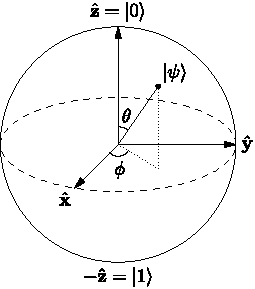
\includegraphics[scale=1.4]{images/Bloch_Sphere.pdf}
    \caption{Rappresentazione generale di un qubit $\ket{\psi}$ sulla sfera di Bloch. Si noti dalla \eqref{generic qubit} come per $\theta = 0$ si abbia $\ket{\psi} = \ket{0} $ (polo Nord) e invece per $\theta = \pi$ risulta $\ket{\psi} = \ket{1}$ (polo Sud).}
    \label{fig:BlochSphere}
\end{figure}

\noindent È fondamentale evidenziare che la rappresentazione dei qubit tramite sfera di Bloch è solo un espediente grafico poiché il prodotto scalare tra qubit è diverso dal classico prodotto scalare di $\mathbb{R}^3$. In $\mathbb{C}^2$ gli stati $\ket{0}$ e $\ket{1}$ sono ovviamente ortogonali, mentre, come evidente dalla figura, su $S^2$ si ha $\braket{0}{1} = -1$. Questo fatto è dovuto ad una sorta di doppio conteggio in \eqref{generic qubit} per la presenza di $\theta/2$.